\documentclass[tikz, border=10pt]{standalone}

% preamble
\usepackage{tikz}
\usepackage{xcolor}
\usepackage{amsmath, amsfonts, amssymb, mathtools}
\usepackage{mathpazo}

% local definition
\def\costhirsty{0.8660256}

% define colors
\colorlet{anglecolor}{green!20}
\colorlet{sincolor}{red}
\colorlet{coscolor}{blue}
\colorlet{tancolor}{orange}

% define styles
\tikzset{
    axe/.style = {},
    important line/.style = {very thick},
    important text/.style = {rectangle, rounded corners, fill=red!10, inner sep=1ex}
}

\begin{document}
    % the graphic
    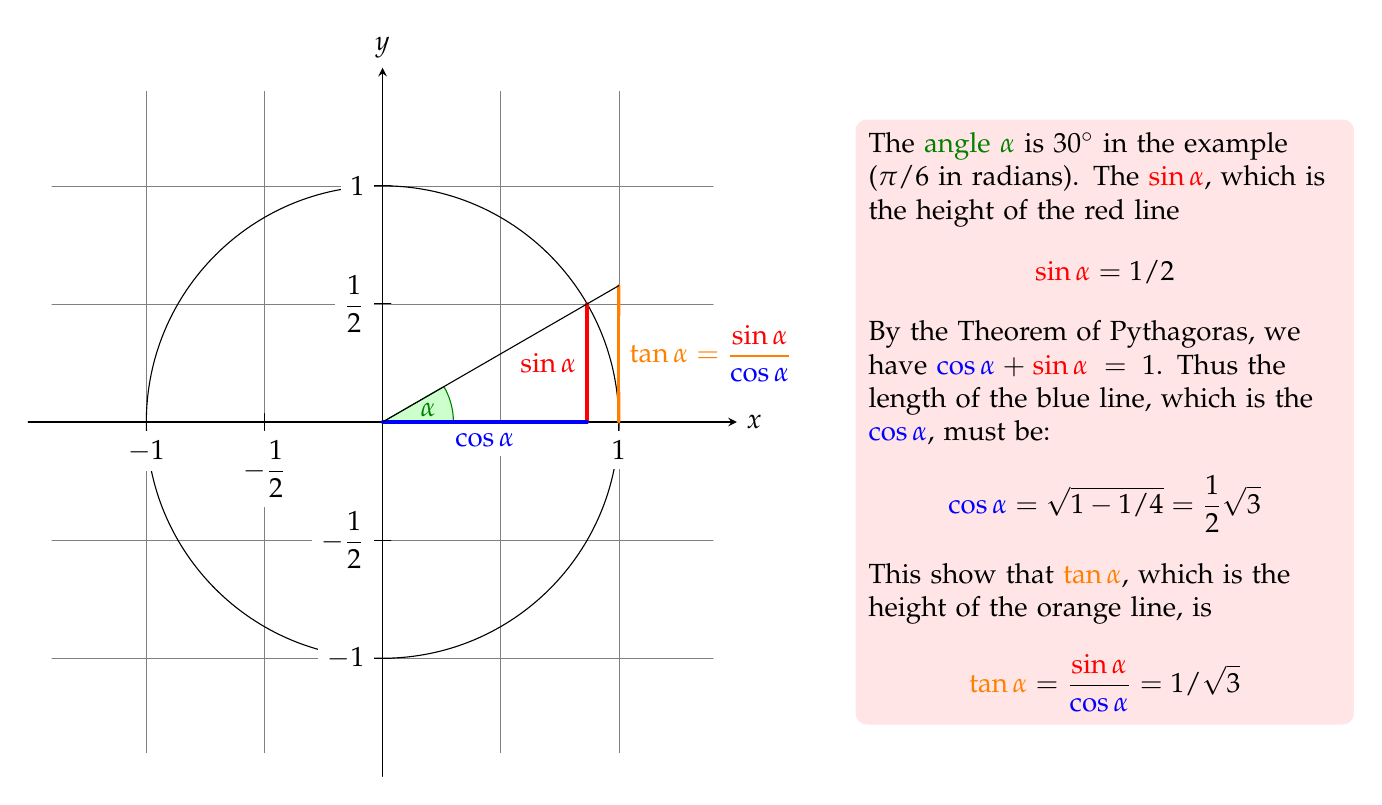
\begin{tikzpicture}[scale=3, cap=round]
        % draw grid lines
        \draw[style=help lines, step=.5] (-1.4, -1.4) grid (1.4, 1.4);
        % draw circle
        \draw (0, 0) circle (1cm);
        % draw axe and sticks
        \begin{scope}[axe]
            % axe
            \draw[->, >=stealth] (-1.5, 0) -- (1.5, 0) node [right]{$x$} coordinate (x axis);
            \draw[->, >=stealth] (0, -1.5) -- (0, 1.5) node [above]{$y$} coordinate (y axis);
            % sticks
            \foreach \x/\xtext in {-1, -0.5/-\dfrac{1}{2}, 1}
                \draw[xshift=\x cm] (0, 1pt) -- (0, -1pt) node [below, fill=white]{$\xtext$};
            \foreach \y/\ytext in {-1, -0.5/-\dfrac{1}{2}, 0.5/\dfrac{1}{2}, 1}
                \draw[yshift=\y cm] (1pt, 0) -- (-1pt, 0) node [left, fill=white] {$\ytext$};
        \end{scope}
        % draw and fill angle
        \filldraw[fill=anglecolor, draw=green!50!black] (0, 0) -- (3mm, 0) arc (0:30:3mm) -- cycle;
        \draw (15:2mm) node[green!50!black] {$\alpha$};
        % draw sine line
        \draw[sincolor, important line] (30:1cm) -- node[left, fill=white]{$\sin\alpha$} (30:1 |- x axis); 
        % draw cosine line
        \draw[coscolor, important line] (0, 0) -- node[below, fill=white]{$\cos\alpha$} (30:1 |- x axis);
        % draw tang line
        \draw[tancolor, important line] (1, 0) -- node[right, fill=white]
            {${\color{tancolor}\tan\alpha} = \dfrac{\color{sincolor}\sin\alpha}{\color{coscolor}\cos\alpha}$}
            (intersection of 0, 0 -- 30:1 and 1, 0 -- 1, 1) coordinate (t);
        % draw line from (0, 0) to (1, tan(\alpha)
        \draw (0, 0) -- (t);
        % draw text block
        \draw [xshift=2cm] node[important text, right, text width=6cm]{
            The {\color{green!50!black} angle $\alpha$} is $30^\circ$ in the example ($\pi/6$ in radians).
            The {$\color{sincolor}\sin\alpha$}, which is the height of the red line
            \[
                {\color{sincolor}\sin\alpha} = 1/2
            \]
            By the Theorem of Pythagoras, we have $ {\color{coscolor}\cos\alpha} + {\color{sincolor}\sin\alpha} = 1$.
            Thus the length of  the blue line, which is the {$\color{coscolor}\cos\alpha$}, must be:
            \[
                {\color{coscolor}\cos\alpha} = \sqrt{1 - 1/4} = \dfrac{1}{2}\sqrt{3}
            \]
            This show that {$\color{tancolor}\tan\alpha$}, which is the height of the orange line, is
            \[
                {\color{tancolor}\tan\alpha} = \dfrac{\color{sincolor}\sin\alpha}{\color{coscolor}\cos\alpha} = 1/\sqrt{3}
            \]
        };
    \end{tikzpicture}
\end{document}